\documentclass[graphics]{beamer}
\usepackage{xcolor}
\usepackage{graphicx}
\usepackage{verbatim}
\usepackage{wrapfig}
\usepackage{tabularx}
\usepackage{multirow}
\usepackage{amssymb}
\usepackage{pifont}
\usepackage{tikz}
\def\Checkmark{\tikz\fill[scale=0.2](0,.35) -- (.25,0) -- (1,.7) -- (.25,.15) -- cycle;} 

\useoutertheme{shadow}
%\usecolortheme{orchid}
\usecolortheme{seahorse}
\newcommand{\cmark}{\text{\ding{51}}}
%\newcommand*{\GtrSim}{\smallrel\gtrsim}

% math commands
\newcommand{\be}{\begin{eqnarray}}
\newcommand{\ee}{\end{eqnarray}}
\newcommand{\beq}{\begin{equation}}
\newcommand{\eeq}{\end{equation}}
\def\simless{\mathbin{\lower 3pt\hbox
      {$\rlap{\raise 5pt\hbox{$\char'074$}}\mathchar"7218$}}}
\def\simgreat{\mathbin{\lower 3pt\hbox
      {$\rlap{\raise 5pt\hbox{$\char'076$}}\mathchar"7218$}}} %> or of order

% variables

\def\toonscale{0.45}
\def\mboxy#1{\mbox{\small #1}}

\defbeamertemplate*{title page}{customized}[1][]
{
  \usebeamerfont{title}\inserttitle\par
  \usebeamerfont{subtitle}\usebeamercolor[fg]{subtitle}\insertsubtitle\par
  \bigskip
  \usebeamerfont{author}\insertauthor\par
  \usebeamerfont{institute}\insertinstitute\par
  \usebeamerfont{date}\insertdate\par
  \usebeamercolor[fg]{titlegraphic}\inserttitlegraphic
}
\begin{comment}
\AtBeginSection[]{
  \frame{
    \frametitle{Outline}
    \tableofcontents[currentsection]
  }
}
\end{comment}


\title{\textcolor{red}{Fast Radio Bursts}}
%\subtitle{}
\author[U. Pen]{{
{ K. Masui, H-S. Lin, J. Sievers}, 
\textcolor{green}{\small Y. Liao, C. Kuo, L. Connor} 
\textcolor{red}{\small U. Pen, T. Chang, X. Chen, J. Peterson and many more}
}
\\[8mm] 
}
\date{December 24, 2015}


\begin{document}

\frame{
\vspace{-0.5in}
\begin{center}  
%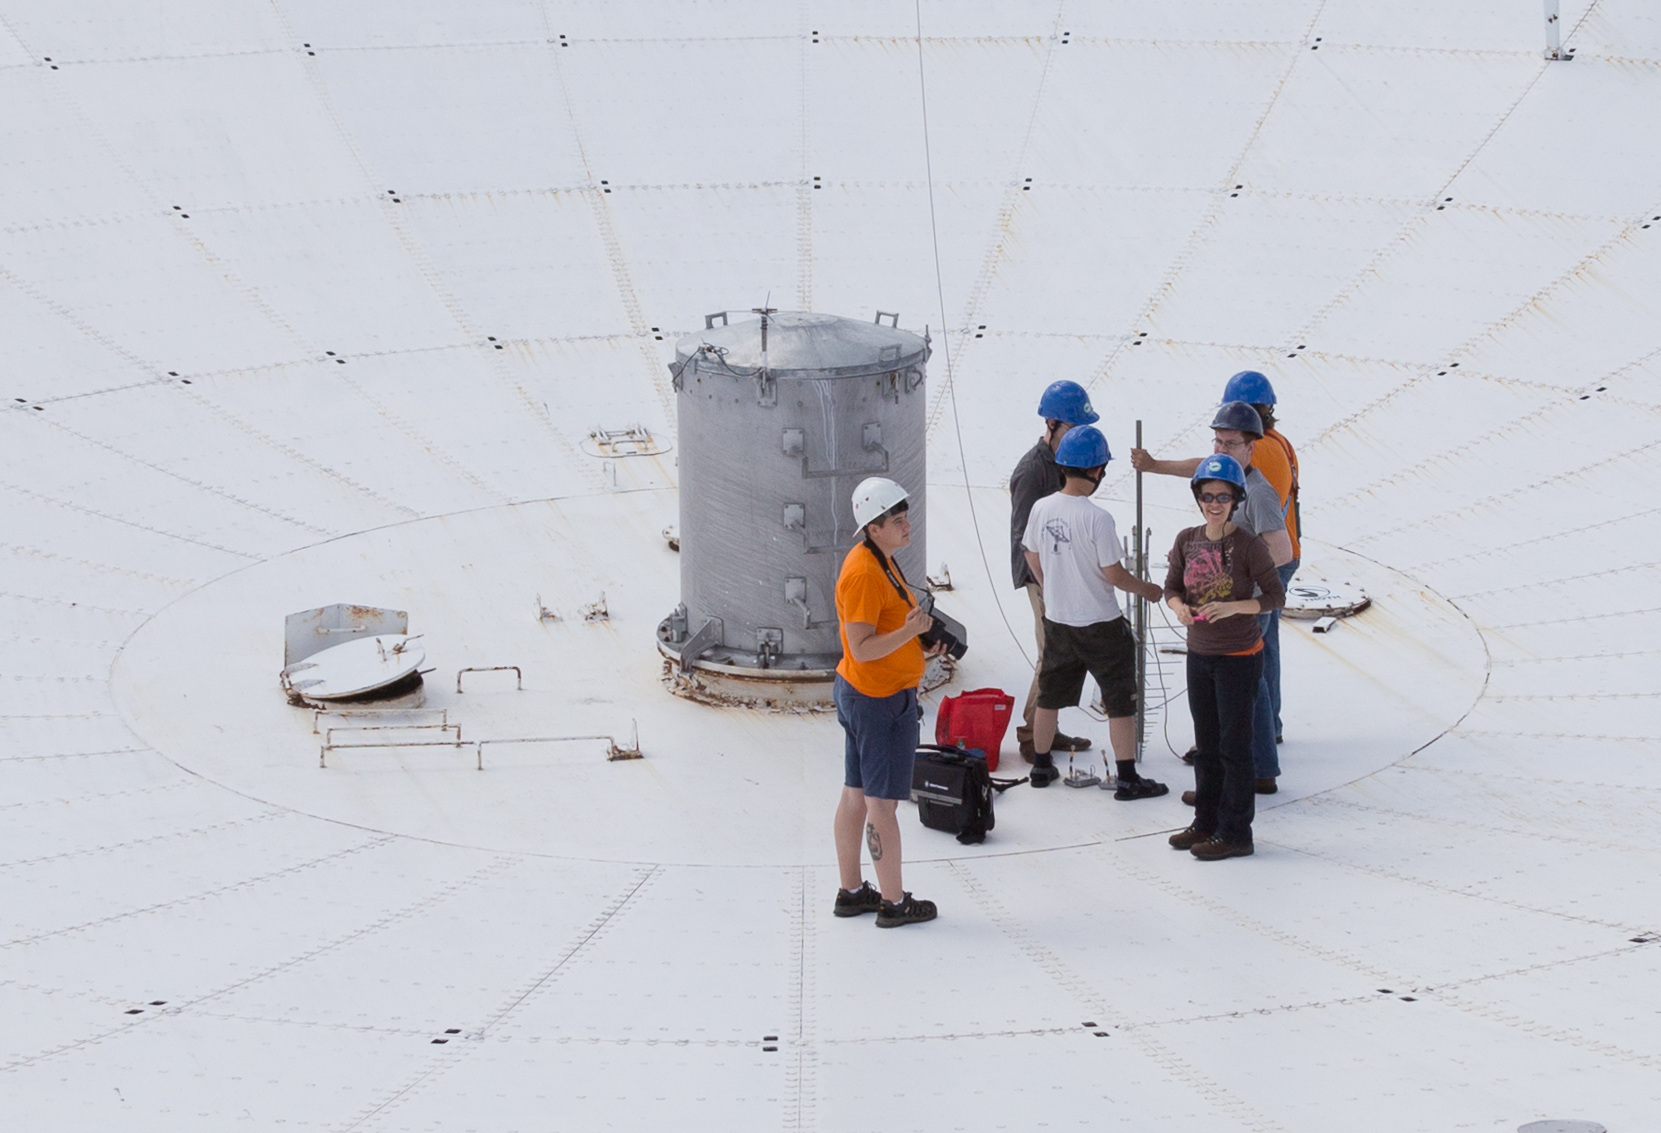
\includegraphics[width=4.4in]{Figures/IMG-0438-by-Andre-cropped.jpg}
\end{center}
\begin{picture}(320,250)
\put(-50,60){
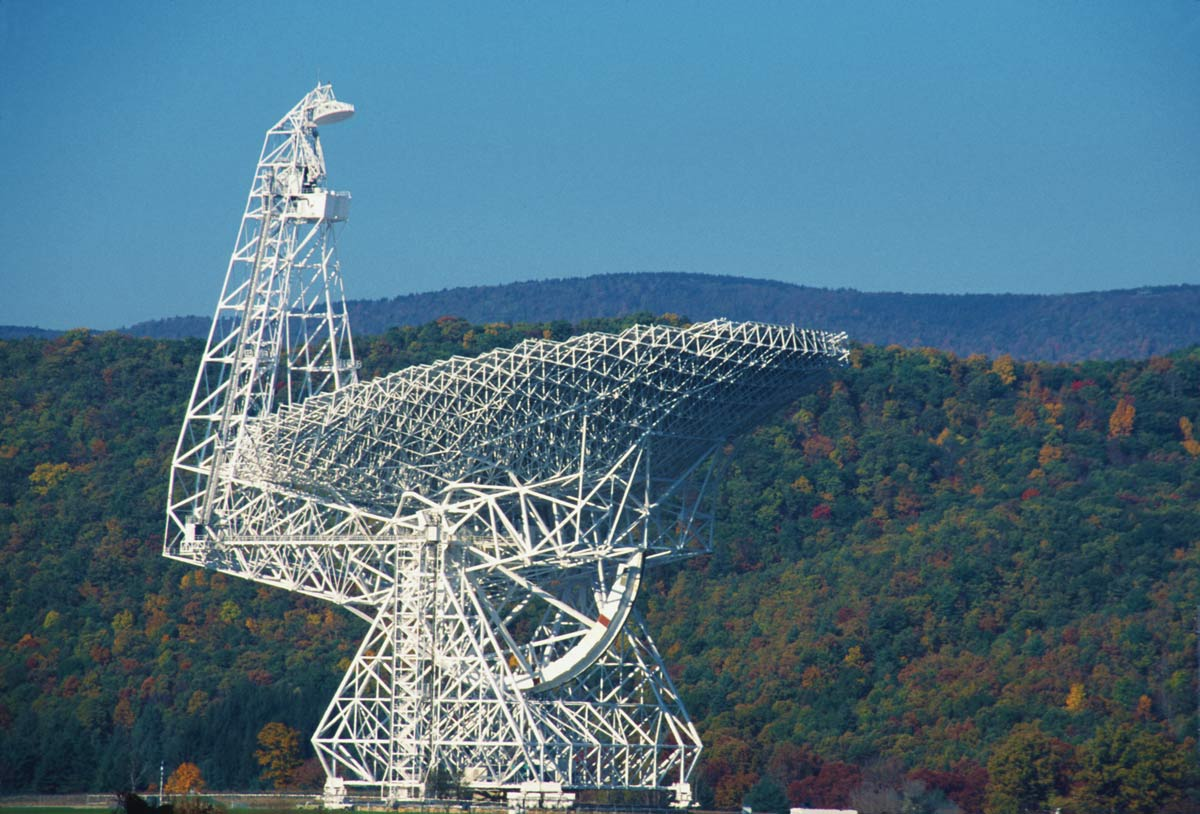
\includegraphics[width=5.5in]{Figures/GBT_nrao.jpg}}
\end{picture}
\vspace{-4in}
\\
image credit: NRAO/AUI/NSF
\\
\vspace{1in}
\titlepage
}

%\section*{Introduction}
\section{Introduction}

\begin{comment}
  \subsection{Outline}

  \frame{
    \frametitle{Outline}
    \tableofcontents
  }
\end{comment}

  \frame{
    \frametitle{Overview}
    \begin{itemize}
      \item FRB
      \item Candidates
      \item Plasma Lensing
      \item Controversies
      \item next steps
    \end{itemize}
  }
\section{FRBs}

\frame{
    \frametitle{FRB}
     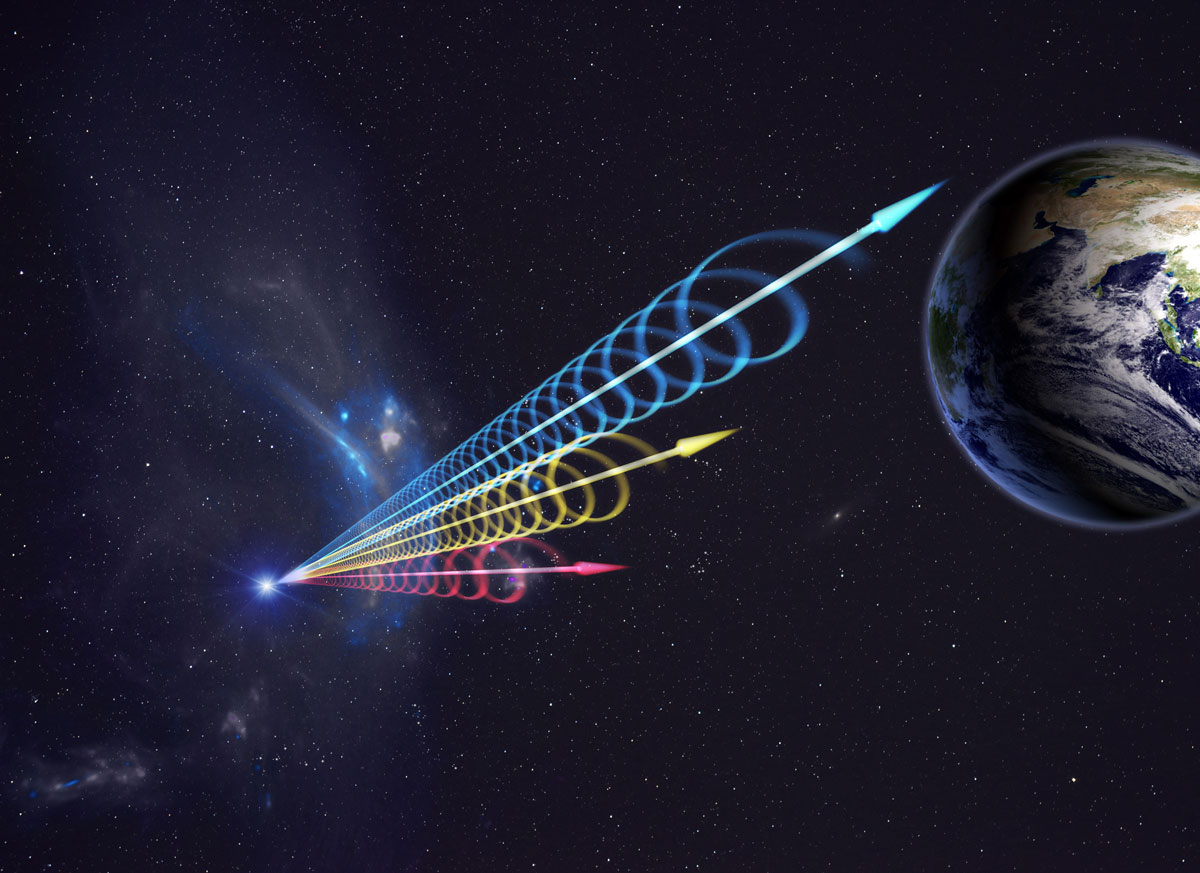
\includegraphics[width=\textwidth]{Figures/FRB_nrao.jpg}
}

\frame{
    \frametitle{FRB110523}
     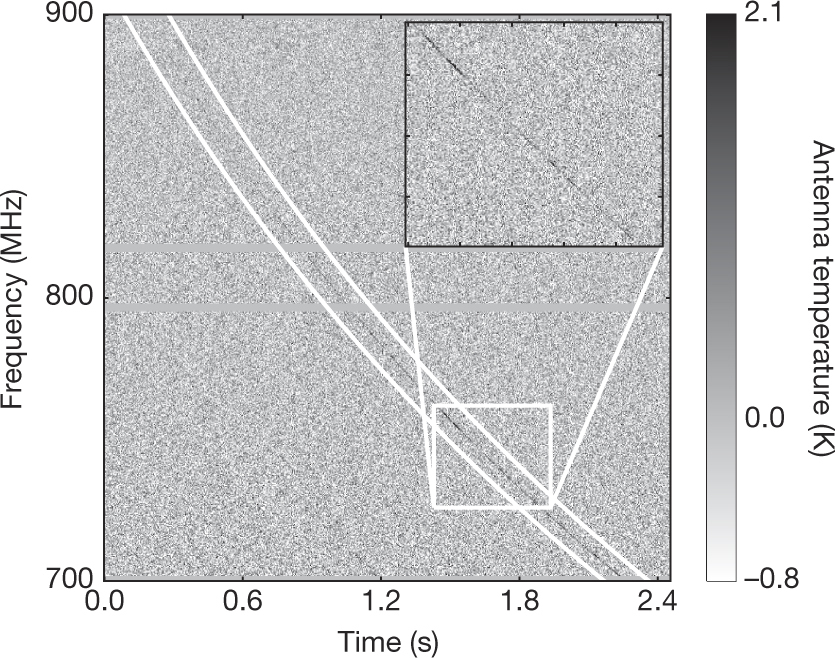
\includegraphics[width=0.8\textwidth]{Figures/nature15769-f1.jpg}

Masui et al 2015, Nature 15769
}

  \frame{
    \frametitle{Basic Properties}
    \begin{itemize}
      \item about 20 FRBs detected
      \item ms duration
      \item some are scattered
      \item some are polarized
      \item high dispersion measure: DM $\sim$ 1000 pc/cm$^3$
      \item likely extragalactic
      \item possibly cosmological $z\sim 1$
      \item duration infers size of 300km  
      \item R-J brightness: $10^{36}$K is $\sim 10^4 T_p$: 
      \item highest brightness temperature in the universe, except
        maybe crab nanoshot
    \end{itemize}
  }


  \frame{
    \frametitle{Candidates}
    \begin{itemize}
      \item cataclysmic: exploding Hawking black holes, merging
        neutron stars, blitzars
      \item repeating: magnetar flares, planet-neutron star, supergiant pulse
      \item local: flare stars, microwave ovens
    \end{itemize}
  }


  \frame{
    \frametitle{Applications}
    \begin{itemize}
      \item misconceptions: cosmological standard ruler, etc
      \item cross correlation analysis: baryonic clustering, cosmic
        magnetic fields (McQuinn 2014)
      \item new high energy phenomena
    \end{itemize}
  }
 
  \frame{
    \frametitle{Candidates}
{%\tiny
\fontsize{0.05cm}{0.055cm}\selectfont 
\begin{table}
\label{TAB-1}
\hspace{-0.5in}   \begin{tabularx}{1.08\textwidth}{@{\extracolsep{\fill}}|lccccccc|}
\hline
\multicolumn{1}{|c}{\textbf{Location}}                                                                                            & \textbf{Model}                                              & \textbf{\begin{tabular}[c]{@{}c@{}}Galactic \\ scintillation\end{tabular}} & \textbf{\begin{tabular}[c]{@{}c@{}}Faraday \\ rotation\end{tabular}} & \textbf{$\mathbf{\frac{dlnN_{\rm FRB}}{dlnS_{\nu}}}$}                                      & \multicolumn{1}{l}{\textbf{Counterpart}}                                    & \textbf{\begin{tabular}[c]{@{}c@{}}DM range\\ (pc cm$^{-3}$)\end{tabular}} & \textbf{\begin{tabular}[c]{@{}c@{}}Pol angle \\ swing\end{tabular}} \\ \hline
\multicolumn{1}{|l|}{\multirow{4}{*}{\begin{tabular}[c]{@{}l@{}}Cosmological \\ (${>} 1 h^{-1}$Gpc)\end{tabular}}}             & Blitzars                                                    & $\times$                                                                         & $< 7$ rad m$^{-2}$                                               & ?                                                                                      & \begin{tabular}[c]{@{}c@{}}gravitational \\ waves\end{tabular}              & 300-2500                                                                & $\times$                                                                  \\
\multicolumn{1}{|l|}{}                                                                                                            & Merging COs                                                 & $\times$                                                                         & $< 7$ rad m$^{-2}$                                      & ?                                                                                      & \begin{tabular}[c]{@{}c@{}}type Ia SNe,\\  X-ray, $\gamma$-ray\end{tabular} & 300-2500                                                                & $\times$                                                                  \\
\multicolumn{1}{|l|}{}                                                                                                            & Primordial BHs                                              & $\times$                                                                         & $< 7$ rad m$^{-2}$                                               & ?                                                                             & $\sim$TeV                                                                   & 300-2500                                                                & $\times$                                                                  \\
\multicolumn{1}{|l|}{}                                                                                                            & Magnetar flare                                              & $\times$                                                                         & $< 7$ rad m$^{-2}$                                               & ?                                                                                      & \begin{tabular}[c]{@{}c@{}}$\sim$ms TeV \\ burst\end{tabular}               & 300-2500                                                                & $\Checkmark$                                                        \\ \cline{1-1}
\multicolumn{1}{|l|}{\multirow{3}{*}{\begin{tabular}[c]{@{}l@{}}Extragalactic, local \\ ($<$200$ h^{-1}$Mpc)\end{tabular}}} & Edge-on disk                                                & $\Checkmark$                                                               & 50-500 rad m$^{-2}$                                                     & -3/2                                                                                   & ?                                                                           & 10-2000                                                                 & ?                                                                   \\
\multicolumn{1}{|l|}{}                                                                                                            & \begin{tabular}[c]{@{}c@{}}Nuclear \\ magnetar\end{tabular} & $\Checkmark$                                                               & 10$^{3-5}$ rad m$^{-2}$                                                 & -3/2                                                                                   & none                                                                        & 10-3000                                                                 & $\Checkmark$                                                        \\
\multicolumn{1}{|l|}{}                                                                                                            & SNR pulsar                                                  & $\Checkmark$                                                               & 20-$10^3$ rad m$^{-2}$                                                  & -3/2                                                                                   & \begin{tabular}[c]{@{}c@{}}archival CC \\ SNe or \\ nearby galaxy \end{tabular}                  & 10$^2$-10$^4$                                                           & $\Checkmark$                                                        \\ \cline{1-1}
\multicolumn{1}{|l|}{Galactic ($< 100$ kpc)}                                                                                & flaring MS stars                                            & $\Checkmark$                                                               & RM$_{\rm gal}$                                                          & -3/2                                                                                   & \begin{tabular}[c]{@{}c@{}}main sequence \\ star\end{tabular}               & $>$ 300                                                           & $\times$                                                                  \\ \cline{1-1}
\multicolumn{1}{|l|}{Terrestrial ($< 10^5$ km)}                                                                             & RFI                                                         & $\times$                                                                         & $<$ RM$_{\rm ion}$                                                          & $\left\{\begin{matrix}-1/2 \,\, if \,\, 2D \\ -3/2 \,\, if \,\, 3D\end{matrix}\right.$ & none                                                                        & ?                                                                       & $\times$                                                                  \\ \hline

\end{tabularx}
\caption{\tiny This table summarizes a number of FRB models by classifying them as cosmological, 
extragalactic but non-cosmological, Galactic, and terrestrial. 
The seven columns are potential observables of FRBs and each
 row gives their consequence for a given model 
 (Blitzars,
 compact object mergers,
 exploding primordial blackholes,
bursts from magnetars,
edge-on disk galaxies,
circumnuclear magnetars,
 supernova remnant pulsars, stellar flares
and terrestrial RFI.
For the latter, we subdivide the RFI into planar RFI (2D) coming
 from the earth's surface, and 3D RFI coming from objects like satellites. 
 Since scintillation
only affects unresolved images, cosmological sources that are not scattered near the source
will not scintillate in our Galaxy, while non-cosmological sources whose screens are intrinsic will. 
For Faraday rotation and scintillation
 we assume 
the RM and SM comes from the same place as the DM, e.g. the IGM for cosmological sources, though such models 
could introduce a more local Faraday effect or a scattering screen.
Even though
all models have to explain the observed 375-1600 pc cm$^{-3}$, some models predict a wider 
range of DM. For instance, in the circumnuclear magnetar or edge-on disk disk scenarios there 
ought to be bursts at relatively low DM that simply have not been identified as FRBs. In our supernova 
remnant model DMs should be very large early in the pulsar's life, though this window is short and 
therefore such high DM bursts would be rare. (from Connor et al 2015)}
\end{table}

}
  }

  \frame{
    \frametitle{FRB110523}
    \begin{itemize}
    \item Masui et al, Dec 2, 2015, Nature 15769
    \item  recorded on May 23, 2011
     \item part of GBT-IM survey, for 21cm intensity mapping (Chang et al 2010,
       Nature, 466, 463)
     \item beat double odds with data: intensity mapping, FRB       
    \end{itemize}
  }
\frame{
    \frametitle{Polarization}
     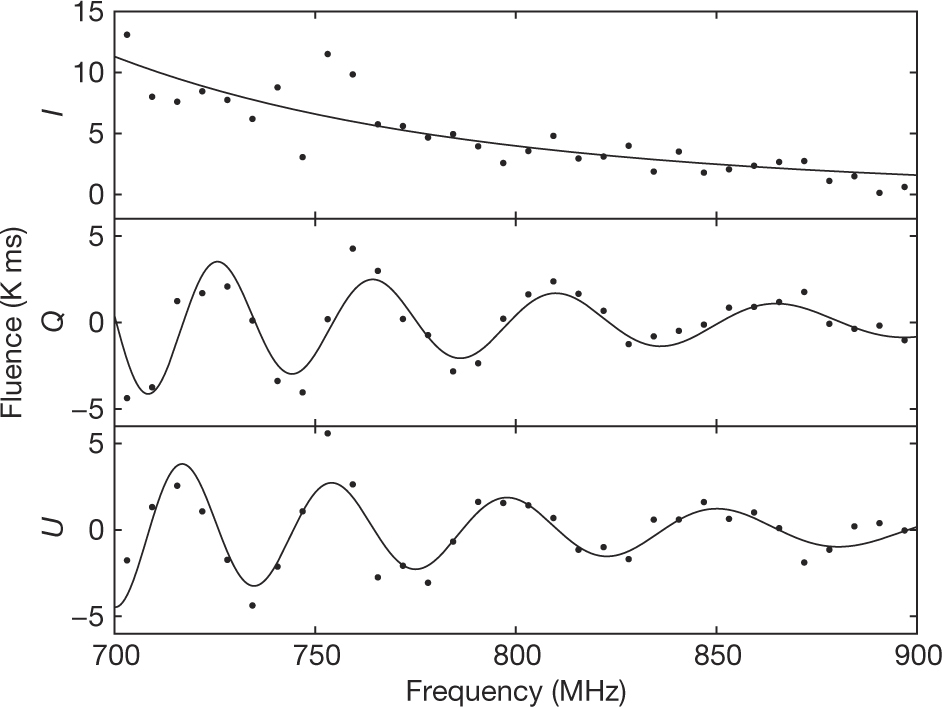
\includegraphics[width=0.8\textwidth]{Figures/nature15769-f2.jpg}
}

  \frame{
    \frametitle{interpretation}
    \begin{itemize}
    \item RM=-186.1 $\pm$ 1.4
    \item galactic+extragalactic RM=18$\pm$3 for this LOS measured from quasars
      (Opperman et al 2015)
    \item $\implies$ magnetic field local to FRB or host galaxy
    \item if DM also local, implies B$\sim  0.3 \mu$G
    \end{itemize}
  }
\frame{
    \frametitle{Angle swing}
     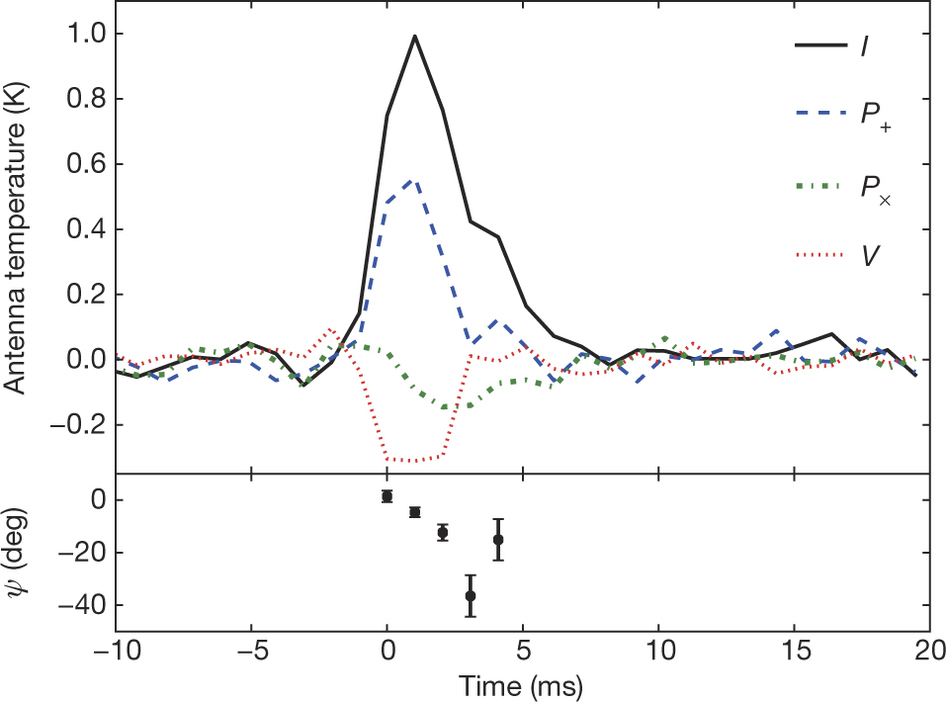
\includegraphics[width=0.8\textwidth]{Figures/nature15769-f3.jpg}
}
  \frame{
    \frametitle{interpretation}
    \begin{itemize}
    \item $5-\sigma$ significance of polarization angle swing
    \item generic for pulsars
    \item unknown for most other processes
    \end{itemize}
  }
\frame{
    \frametitle{Scattering}
     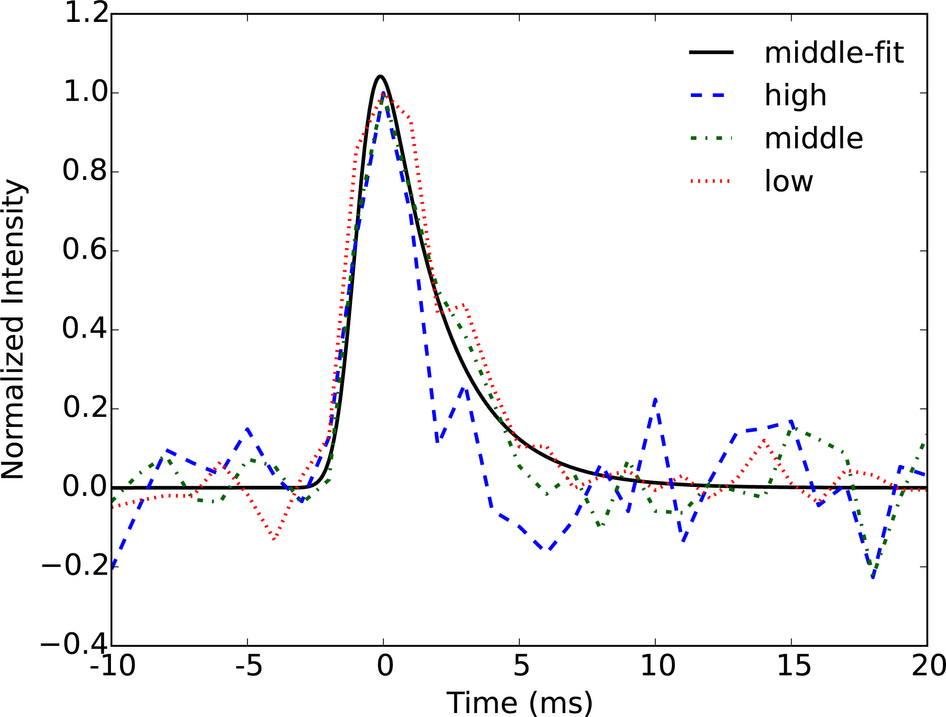
\includegraphics[width=0.8\textwidth]{Figures/nature15769-sf2.jpg}
}
  \frame{
    \frametitle{interpretation}
    \begin{itemize}
    \item ms scattering is generally due multipath propagation
    \item location was once thought to be IGM
    \item FRB110523 shows $\mu$s scintillation from Galactic multipath
    \item scattering tail scintillates!
    \item {\it stars twinkle, planets don't}
    \item constrains source size less than $\sim$ microarcsecond
    \item scattering screen is physically associated with FRB, not intergalactic
    \end{itemize}
  }
\frame{
    \frametitle{inferred properties}
     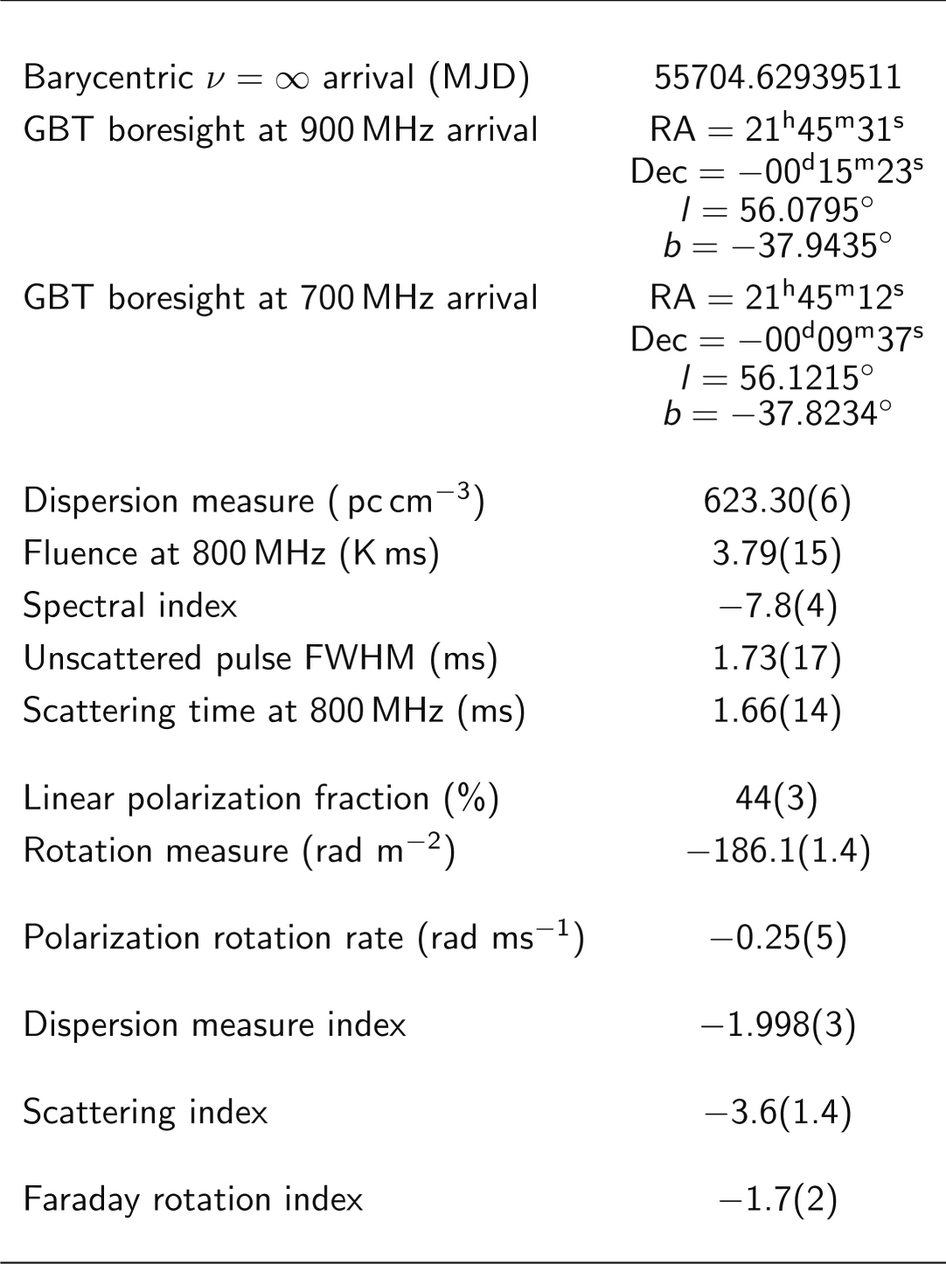
\includegraphics[width=0.5\textwidth]{Figures/nature15769-st1.jpg}
}
  \frame{
    \frametitle{more interpretations}
    \begin{itemize}
    \item flare stars ruled out: not enough deviation from $\lambda^2$
      law, lower bound of plasma cloud $R>10$AU, bigger than any
      plausible star
    \item scattering index consistent with refractive lensing scaling
      (Pen\&Levin 20134
    \end{itemize}
  }


\section{Summary}
  \frame{
    \frametitle{Looking forward}
    \begin{itemize}
      \item how do we reduce the allowed model space?
      \item 1. repeat rate (Connor et al 2015)
      \item 2. host galaxy
      \item 3. precision localization within host: nuclear, SNR, SFR?
      \item more unpublished bursts with new claims
      \item thousands of bursts with GBT-MB, CHIME, HIRAX, UTMOST
      \item localization with VLBI
    \end{itemize}
  }

\frame{
    \frametitle{repeat rates}
     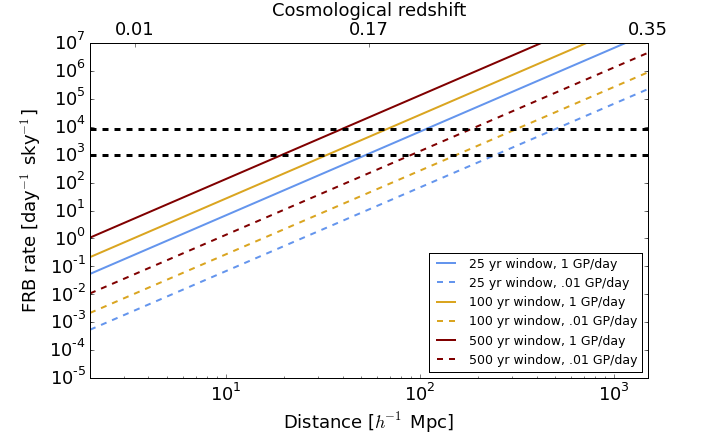
\includegraphics[width=\textwidth]{Figures/FRB_SNR_rate.png}

     Connor, Sievers, Pen 2015
}



  \frame{
    \frametitle{Conclusion}
    \begin{itemize}
      \item most plasma properties due to local environment, not
        cosmological
      \item FRBs likely extragalactic, but not cosmological        
      \item ISM structure: mapping cosmic plasma and magnetic fields
    \end{itemize}
  }

\end{document}
